\documentclass[a4paper,12pt]{amsart}
\usepackage{amssymb,latexsym,amsmath}
\usepackage[T1]{fontenc}
\usepackage[utf8]{inputenc}
\usepackage{tikz}
\usetikzlibrary{patterns}
\usetikzlibrary{arrows.meta}
\usepackage{color}

\begin{document}

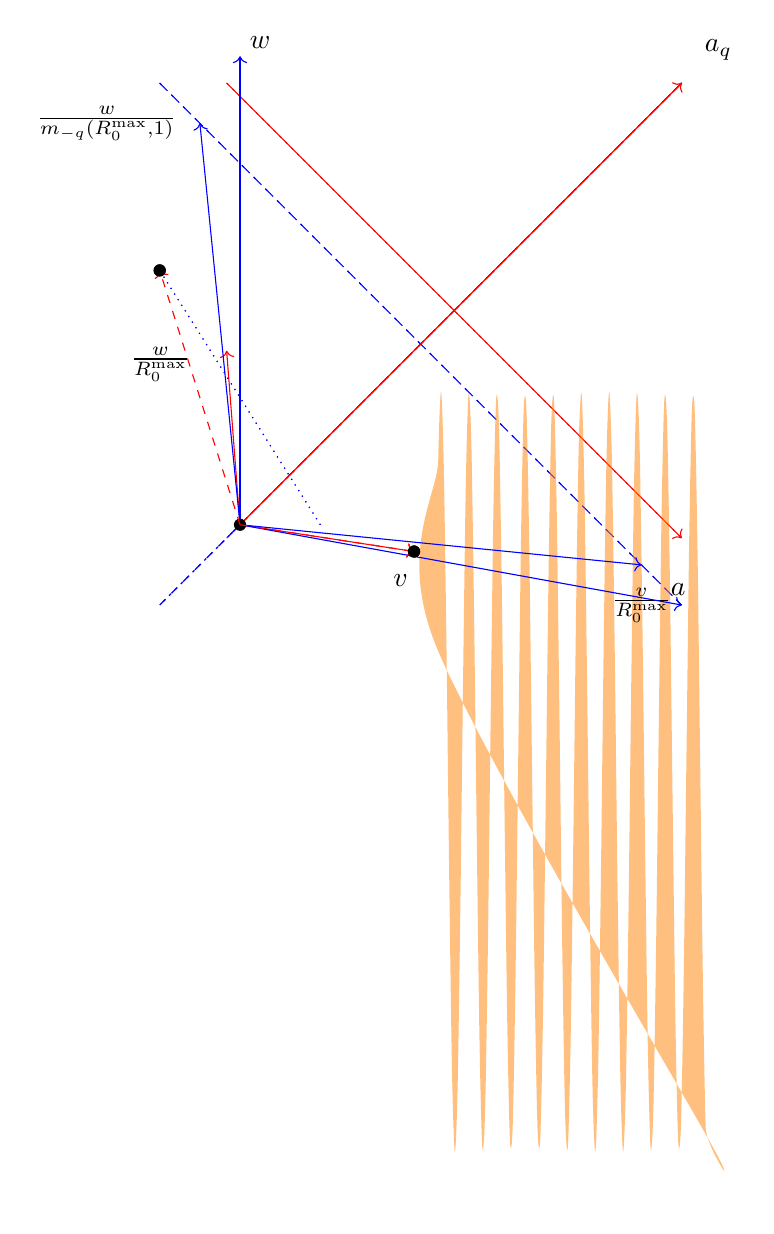
\begin{tikzpicture}[scale=1.7]
	\draw[dashed,red] (-0.1,-0.1)--(3.3,3.3);
	\draw[red,dashed,dash pattern=on 1pt off 2pt] (-0.1,3.3)--(3.3,-0.1);
	\draw[->,red] (-0.1,3.3)--(3.3,-0.1);
	\draw[dotted,blue] (0.6,0)--(-0.6,1.9);
	\draw[dashed,blue] (-0.6,-0.6)--(3.3,3.3);
	\draw[dashed,blue] (-0.6,3.3)--(3.3,-0.6);
	\draw[dashed,blue,dash pattern=on 1pt off 2pt] (3.3,3.3)--(-0.6,-0.6);
	\draw[dashed,blue,dash pattern=on 1pt off 2pt] (-0.6,3.3)--(3.3,-0.6);
	\fill[orange,fill opacity=0.5] plot [smooth cycle,samples=100,domain=1.46:3.5] (\x,{1.42*(cos(30*\x r)+sqrt(3)*sin(30*\x r)-1.3)});
	\draw[->,red] (0,0)--(1.3,-0.2);
	\node at (1.2,-0.3)[anchor=north]{$v$};
	\draw[->,red] (0,0)--(-0.1,1.3);
	\node at (-0.3,1.2)[anchor=east]{$\frac{w}{R_0^{\max}}$};
	\draw[->,blue] (0,0)--(3,-0.3);
	\node at (3,-0.4)[anchor=north]{$\frac{v}{R_0^{\max}}$};
	\draw[->,blue] (0,0)--(-0.3,3);
	\node at (-0.4,3)[anchor=east]{$\frac{w}{m_{-q}(R_0^{\max},1)}$};
	\draw[->,blue] (0,0)--(0,3.5);
	\node at (0,3.6)[anchor=west]{$w$};
	\draw[->,red] (0,0)--(3.3,3.3);
	\node at (3.3+0.1,3.3+0.1)[anchor=south west]{$a_q$};
	\draw[->,blue] (0,0)--(3.3,-0.6);
	\node at (3.3+0.1,-0.6)[anchor=south east]{$a$};
	\draw[dotted,blue] (0.6,0)--(-0.6,1.9);
	\fill[black,fill opacity=1.] (0,0) circle (1.3pt);
	\fill[black,fill opacity=1.] (1.3,-0.2) circle (1.3pt);
	\fill[black,fill opacity=1.] (-0.6,1.9) circle (1.3pt);
	\draw[->,dashed,red] (0,0)--(-0.6,1.9);
	\draw[->,dashed,red] (0,0)--(1.3,-0.2);
	\fill[black,fill opacity=1.] (1.3,-0.2) circle (1.3pt);
	\fill[black,fill opacity=1.] (-0.6,1.9) circle (1.3pt);
	\end{tikzpicture}

\end{document}